\documentclass{llncs} 

\usepackage{verbatim}
%\usepackage[pdfpagescrop={92 112 523 778},a4paper=false]{hyperref}
\usepackage{hyperref}
\usepackage[pdftex]{graphicx}
\hypersetup{
    pdftitle={FOAF+SSL: RESTful Authentication for the Social Web},
    pdfauthor={Henry Story, Bruno Harbulot, Ian Jacobi, Mike Jones},
    pdfkeywords={}
}

\graphicspath{{figures/}}
\urlstyle{sf}

\usepackage[hyper]{listings}
\lstset{basicstyle=\rm\footnotesize\ttfamily,frame=tbrl,showstringspaces=false,columns=fixed,basewidth=0.55em}

\sloppy
\clubpenalty=50000
\widowpenalty=50000

%% To comment out for the final version
\newcount\hour
\newcount\minute
\def\Time{\hour=\time
          \minute=\time
          \divide\hour by60
          \ifnum\hour<10 0\fi\number\hour:%
          \multiply\hour by60
          \advance\minute by -\hour
          \ifnum\minute<10 0\fi\number\minute%
         }
\RequirePackage{rotating}
\RequirePackage{graphicx}
\RequirePackage{prelim2e}[1996/01/01]
\renewcommand*{\PrelimText}{%
	\hskip -1.2cm plus -\marginparsep
    \begin{rotate}{90}
       \rlap{%
          \scalebox{0.75}{\textnormal{%\texttt{Draft: \today\ -- \Time -- Page \thepage}
          This article is available under the ``Attribution 3.0 Unported'' Creative Commons License.}}
       }%
    \end{rotate}
    \hskip 0pt plus 1filll
 }
%%%%%%%%%%%%%%%%%%%%%%%%
\newcounter{custompropcounter}
\newenvironment{customprop}[1]
{\refstepcounter{custompropcounter}\label{#1}%
\vspace{0.31cm}
\tabular{p{.08\textwidth}p{.91\textwidth}}
{\bf (P\arabic{custompropcounter})} & 
\minipage{\textwidth}
\footnotesize}
{\endminipage
\endtabular\vspace{0.31cm}}

\newcounter{customrelcounter}
\newenvironment{customrel}[1]
{\refstepcounter{customrelcounter}\label{#1}%
\vspace{0.31cm}
\tabular{p{.08\textwidth}p{.91\textwidth}}
{\bf (R\arabic{customrelcounter})} & 
\minipage{\textwidth}
\footnotesize}
{\endminipage
\endtabular\vspace{0.31cm}}

\newcounter{customdefcounter}
\newenvironment{customdef}[1]
{\refstepcounter{customdefcounter}\label{#1}%
\vspace{0.31cm}
\tabular{p{.08\textwidth}p{.91\textwidth}}
{\bf (D\arabic{customdefcounter})} & 
\minipage{\textwidth}
\footnotesize}
{\endminipage
\endtabular\vspace{0.31cm}}

\begin{document}
\title{FOAF+SSL: RESTful Authentication for the Social Web\footnote{This paper is licensed under the Creative Commons Attribution 3.0 unported license described at \url{http://creativecommons.org/licenses/by/3.0/}}}
\author{Henry Story\inst{1} \and Bruno Harbulot\inst{2} \and Ian Jacobi\inst{3} \and Mike Jones\inst{2}}
\institute{Sun Microsystems, 
\url{http://blogs.sun.com/bblfish}
\and
The University of Manchester, UK,
\email{Bruno.Harbulot@manchester.ac.uk}
\and
MIT}

\maketitle
\begin{abstract} 
 We describe a simple protocol for RESTful authentication, using
 widely deployed technologies such as HTTP, SSL/TLS and Semantic Web
 vocabularies.  This protocol can be used for one-click sign on to web sites using existing 
 browsers ---~requiring the user to enter neither an identifier nor a password.  Upon this, distributed, open yet secure social networks and applications can be built.  After summarizing each of these technologies and how
 they come together in FOAF+SSL,\footnote{Up-to-date information on
   developments in this protocol are available at
   \url{http://esw.w3.org/topic/foaf+ssl}.} we describe declaratively the
 reasoning of a server in its authentication decision. Finally, we compare this protocol to 
 others in the same space.
\end{abstract}
\section{Introduction}

Many services that require authentication rely on centralized systems.
  The identity of the user is constrained
to that administrative domain, forcing her to have a different account and identifier
for each organization she interacts with. This inability to relate identities easily across
domains also makes the creation of links between people in distinct organizations 
difficult.

Every time a person needs authenticated access to a new
organization, a new registration needs to be made; this is a burden
for both the user and the organization. The process of registration is
either (a) minimal ---~for example, e-mail address confirmation~---, or
(b) more formal ---~for example, in a workplace, where an
administrator has to create an account after making verifications
out-of-band. Process (a) is lightweight, but will often provide
insufficient information, whereas process (b) may initially be able to give more
information about a user, at the expense of a costly
verification phase during the registration.

Attempts to decentralize this process have been
made. Shibboleth,\footnote{\url{http://shibboleth.internet2.edu/}} for
example, aims at sharing accounts across administrative boundaries;
however, it relies on a rigid federation process between
organizations.  OpenID, enables authenticating a user against a URI,
but does not build a social web on that. Neither Shibboleth nor OpenID fully comply with web architecture principles (see Section~\ref{sec:rest} on REST), which in part explains their limitations.

This paper describes a novel approach that relies on combining the use
of SSL client certificates and Semantic-Web-based FOAF networks. The
result is a secure, open and distributed authentication mechanism,
which is able to satisfy simple requirements ---~such as authenticating
a user by URI, like OpenID, but without the user needing to remember this URI~--- 
as well as more complex requirements, where the authorization to a service 
depends on distributed properties of the user, such as his position 
in a social network. This proposal is built on
a RESTful architecture, the same that underpins the
largest and most successful network of distributed linked information,
the Web.

Section~\ref{sec:background} introduces the background technologies of
the Semantic Web and FOAF, as well as cryptography and
client-certificate authentication.  Section~\ref{sec:foaftlsprotocol}
presents the FOAF+SSL protocol.  Section~\ref{sec:other} compares this
approach to others.

\section{Background}
\label{sec:background}

\subsection{The RESTful Web Architecture}
\label{sec:rest}

{\em Representational State Transfer} (REST)~\cite[Chap.~5]{fielding2000phd}
is an architectural style for
building large-scale distributed information networks, the most famous
of these being the World Wide Web~\cite{WebArchVol1}.  To build such a
network requires that each of the parts be able to grow independently
of any of the others, with very little central coordination, and that
each of the resources thus created be able to refer easily to any of
the others.
%
The logical building blocks for this are the following:
\begin{enumerate}
\item The specification of universal names, also known as Universal
  Resource Identifiers (URIs) --- such as the familiar Universal Resource Locators (URLs).
\item The mapping of URIs to Resources, also known as the reference relation.
\item Canonical methods for manipulating the resources mapped by each
  URI, via {\em representations} of the resource.  Such a protocol
  specifies a canonical dereferencing mechanism, enabling a holder of
  a URI to find and manipulate the resource referred to by that URI.
  {\tt http://...} URLs use the HTTP protocol as their dereferencing
  mechanism, for example.  By sending a GET request to the object at a given HTTP
  URL, a  {\em
    representation} of the resource is returned.  A resource can
  be created,  changed, and deleted using the POST, PUT, and DELETE methods 
  respectively.
  \end{enumerate}

REST specifies the architectural style required to build such a
protocol with the aim of maximum networkability; that is, any
representation should be able to link to any resource from anywhere,
using the URI alone to do so.

\subsection{The Semantic Web}

Whereas URLs in the initial web of hyperlinked documents referred only
to documents, the Semantic Web specifies how to extend this to enable
a web of resources. In the Semantic Web, it becomes
possible for URLs to refer to anything, be it:
\begin{enumerate}
\item physical things ---~for example, {\tt
  <https://romeo.example/\#i>}
may refer to a human named Romeo;
\item relations between two individuals ---~for example, the relation of
  knowing someone which {\tt <http://xmlns.com/foaf/0.1/knows>} refers
  to; or
\item classes ---~for example, people may be described as being instances of {\tt
  <http://xmlns.com/foaf/0.1/Person>}, the set of persons.
\end{enumerate}

The meaning of these URLs can be found by dereferencing them using
their canonical protocol. Thus, doing an HTTP GET on {\tt <http://xmlns.com/foaf/0.1/knows>} should return a
representation describing it. Since HTTP is built to allow content
negotiation, well configured web servers will return the representation best
fitting the client's needs. Entering the above URL in a web browser
will return a human readable HTML page describing the `knows'
relation. A Semantic Web agent could ask for the standard
machine-friendly RDF representation.

A Semantic Web document is a serialization of a graph of directed
relations between objects. Each relation exists as a triple of {\tt
  <subject> <relation> <object>}, where each of {\tt subject}, {\tt
  relation} and {\tt object} can be chosen among any of the URIs or string literals. Since it is tedious to read
and write such URLs, this article uses the N3\footnote{Current N3
  tutorial at:
  \url{http://www.w3.org/2000/10/swap/doc/Overview.html}.} {\tt
  @prefix} notation. The following prefixes will be used throughout
this article:

\begin{lstlisting}[basicstyle=\rm\scriptsize\ttfamily]
@prefix log: <http://www.w3.org/2000/10/swap/log#> .
@prefix dc: <http://purl.org/dc/elements/1.1/> .
@prefix cert: <http://www.w3.org/ns/auth/cert#> .
@prefix rsa: <http://www.w3.org/ns/auth/rsa#>
@prefix foaf: <http://xmlns.com/foaf/0.1/> .
@prefix rdfs: <http://www.w3.org/2000/01/rdf-schema#> .
@prefix owl: <http://www.w3.org/2002/07/owl#> .
@prefix romeo: <https://romeo.example/#> .  #see RFC2606 on .example domains
@prefix jult: <https://juliet.example/#> . 
@prefix : <> . # special vocabulary defined for this paper 
\end{lstlisting}

Thus, to say ``Romeo is a person'', one can write: {\tt romeo:i a foaf:Person.}. Since
each of the resources in that sentence is named by a URL, one can GET further information about each by dereferencing it, and if that representation itself contains relations do the same recursively. This is known as Linked Data\footnote{see Tim Berners-Lee's note  \url{
http://www.w3.org/DesignIssues/LinkedData.html}}.

Each representation returned by a resource can be interpreted as a
graph of relations, which can be isolated in N3 by placing them within
curly brackets {\tt \{ \}}.\footnote{Unlike the Named Graph
brackets in SPARQL; N3 supports anonymous graphs.}  The
relation that maps a resource to the graph described by the document retrieved using the
canonical dereferencing method of its URI  is defined as the {\tt :semantics} relation. Thus,
after dereferencing {\tt romeo:i}, one may state the following, without asserting the
actual statements within the brackets as true:

\begin{customprop}{prop:romeoSem}
\begin{verbatim}
	romeo:i :semantics { romeo:i a foaf:Person;
	                         :hasPrivateKeyFor pubKey;
	                         foaf:name "Romeo";  
	                         foaf:knows  jult:me . }
\end{verbatim}
\end{customprop}


%Of special note here is the introduction of curly-brackets to the more
%familiar syntax of N-Triples or Turtle. 
%In particular, curly-brackets are used to enclose a particular graph of triples such that the graph may be
%related to other properties.

These graphs can also be used to formulate rules, as when we define the
above {\tt :semantics} relation in terms of the established {\tt
  log:semantics} property, which relates a document to its graph, and {\tt :representation} 
relating a resource to one of its representations (the {\tt?} prefixed variables are universally quantified):

\begin{customdef}{def:representation}
\begin{verbatim}
	{ ?resource :representation ?doc . ?doc log:semantics ?graph . } 
	      => { ?resource :semantics ?graph . }
\end{verbatim}
\end{customdef}


The {\tt log:} namespace\footnote{The {\tt log:} namespace is
  described at \url{http://www.w3.org/DesignIssues/N3Logic}.} tends to
make significant use of enclosed graphs, or ``formulas''.
In particular, the {\tt log:includes} property links a subject graph to an object
graph by asserting that the latter is a subset of the former graph;
the {\tt log:implies} property, also written as {\tt =>}, can
serve as the basis for reasoning based on first-order logic (with the
introduction of appropriate variables).

Even though the Semantic Web is built in order to make merging of
information easy, it is not a requirement to do so. We will be using
this notation to help illustrate clearly when 
merging graphs is reasonable.

\subsection{FOAF, reputation networks and the Web of Trust}

{\em FOAF},\footnote{Defined at \url{http://xmlns.com/foaf/0.1/}.}
short for Friend-of-a-Friend, is an RDF vocabulary used to describe
people, agents, groups and their relations. When
used on the Semantic Web, this allows each person to describe himself 
and his network of friends.

By giving oneself a URI ---~{\em aka.} a Web ID~---, one can describe one's
personal social network by linking oneself to acquaintances by
reference. 
Someone who has been given the {\tt romeo:i} URL
by Romeo himself, and then fetched its {\tt :semantics} (ending up with the
statements in P\ref{prop:romeoSem}) has
good reason to trust that the information there is correct
and, thus, to merge it (in a defeasible manner) with his own belief
store. This graph itself will contain further URIs, such as {\tt
  jult:me}, whose {\tt :semantics} the agent can also GET. 
Similarly, the user can then add {\tt romeo:i} to his FOAF file, to publish
{\tt :me foaf:knows romeo:i}.

Thus, a peer-to-peer information network can be built, where each person
specializes in keeping up-to-date the information they feel
responsible for, linking to the best sources for objects they
do not wish to maintain. In return, as the quality
of one's information and links increases, others feel more confident
linking to it, reducing their own work and responsibilities.

As the network grows, the
value of the network grows exponentially, as predicted by Metcalf's
Law~\cite{SemWebMetcalf}, creating a virtuous circle.  Current social 
networking sites, such as Facebook and LinkedIn, to name a few among many, 
have shown how this can work in less distributed settings, taking advantage of the same law.

The plain {\tt foaf:knows} relation may be enhanced with trust descriptions so as to create a {\em
  reputation network}~\cite{DBLP:conf/www/GolbeckPH03}, and, in the
case of FOAF+SSL, this trust can be backed by the use of cryptographic
keys and signatures, so as to form a secure Web of Trust (as described
in the next sections).

\subsection{Public key cryptography}

{\em Public key cryptography} allows two peers to communicate securely
without requiring them to share a secret, through
the use of unique pairs of keys.  One key, called the {\em public
  key}, may be disseminated widely, and the other, the {\em private
  key}, is to be kept only by its owner.
This is in contrast to symmetric cryptography, where both
participants must share the knowledge of the same {\em secret} key for
both encryption and decryption.

Public key cryptography relies on the conjecture that it is infeasible
to obtain any private key that corresponds to a given public key
through brute force because this
operation is too computationally expensive.  It also assumes that no
two distinct individuals will generate the same key-pair randomly. We can 
define in D\ref{def:hasPrivateKeyFor} an inverse functional property
{\tt :hasPrivateKeyFor}.

\begin{customdef}{def:hasPrivateKeyFor}
\begin{verbatim}
 :hasPrivateKeyFor a owl:InverseFunctionalProperty;
        rdfs:domain foaf:Agent;
        rdfs:range cert:PublicKey .
\end{verbatim}
\end{customdef}

Thanks to the dual-nature of the public and private key pair, two
distinct actions are made possible:

\begin{enumerate}
\item
{\em Encryption} is the obfuscation of a plain text message, generating a
scrambled message using the public key of a key pair,
so that it may only be decrypted using the corresponding private key.
\item
{\em Signing} is the process of associating a digital signature with a
message; this signature is generated using a private key. The
authenticity and integrity of the message can then be verified using
the corresponding public key.
\end{enumerate}

A {\em public key certificate} is the signed combination of a public
key and some information related to this key. Such a certificate may
be self-signed (using the private key that matches the public key it
contains) or signed by a third party. The party that signs a certificate 
(self-signed or not) endorses its contents.
Trusting the party that signed a certificate can be a reason for believing its contents.

Two different architectures have been developed to make use of third
party signing of public key certificates: the hierarchical Public Key
Infrastructure (Section~\ref{sec:pkix}) and the cryptographic Web of
Trust (Section~\ref{sec:wot}).  In both architectures, an application
or hosting environment is initially configured with a trusted set of
certificates known as {\em trust anchors}.  When presented with an
unknown certificate, an application verifies its authenticity by attempting 
to build a certification path --- or chain ---
between the certificate and one of the trust anchors. A certificate
becomes trusted if and only if it has been signed using a certificate
which is already trusted. If necessary, this operation may be repeated
to build a path through intermediate certificates, through which the
trust relation is transitive.

%Usually, the successful verification of a new certificate
%implies the establishment of only a temporary level of trust of the other party for the duration of some operation performed with the certificate. Applications may also, through some external mechanism,
%add some certificate to their set of trust anchors explicitly.

The hierarchical Public Key Infrastructure model and the cryptographic
Web of Trust model mainly differ in the way in which certificates are
distributed and intermediates are trusted. In both cases, the initial
establishment of trust (i.e. the selection of trust anchors) requires
an initial import of certificates which is out of band, but this
process is much less onerous than obtaining all public key
certificates for all entities likely to take part in secure
communications.


\subsection{PKI and hierarchical model of trust}
\label{sec:pkix}

The {\em Internet X.509 Public Key Infrastructure}~\cite{rfc5280}
(PKI) is a hierarchical model for distributing and trusting
certificates. In this model, certificates are signed by a {\em
  certification authority} (CA). X.509 certificates incorporate a {\em
  Subject Distinguished Name} (Subject DN), which identifies the
subject of the certificate, and an {\em Issuer Distinguished Name}
(Issuer DN), which identifies the issuer of the certificate --- 
the entity that signs the certificate . An X.509
certificate may only have one Issuer DN, which must be the Subject DN
of the certificate that has been used to issue it. This structure builds
a hierarchical tree from the root CA certificate, via optional intermediate
CA certificates, to the end-entity (i.e. client or server) certificates.

Most web-browsers and operating systems provide a default list of CA certificates which
they make their users trust implicitly. This list can usually be changed
by the user, a feature often used by institutional PKIs.

\subsection{Cryptographic Web of Trust}
\label{sec:wot}

The cryptographic {\em Web of Trust} (WoT) is a form of public key
infrastructure (although rarely called PKI) where each
participant may assert trust in any other participant, without a
specific hierarchy.

The Web of Trust model is used by PGP; what is often referred to as a
{\em PGP public key} is, in fact, a form of a public key certificate,
since it also contains additional information (such as an e-mail
address) and is signed so as to assert its authenticity. Such a
certificate is self-signed, but may also contain additional signatures
--- those by whom the association between the key and this additional
information is trusted.

In PGP, the trust anchors are the user's own certificate and the
certificates the user trusts, some of which may be from trusted
introducers (that is, people through whom trust is transitive).
The number a signatures a certificate has reflects the connectivity
to other parties. The more signatures a certificate has, the
more likely it is that a third party will be able to find a certification
path to that certificate via trusted introducers.

%Key-signing parties ---~where some out-of-band form of verification (e.g. with a passport) is
%done prior to signing a certificate~--- are often used for adding new trust anchors.
%If a
%participant, $A$, checks the identity of participant $B$, then $A$ may
%opt to sign $B$'s certificate, thus asserting to any third
%party who may have $A$ as a trusted introducer that the information in
%$B$'s certificate is accurate.  Furthermore, direct trust may now be
%established in future communications between $A$ and $B$ through the
%use of public-key encrypted communications.
%
%If $A$ also trusts $B$ to make reasonable decisions in what
%certificates $B$ signs, $A$ can also add $B$ as a trusted introducer,
%so that $A$ can trust the certificates that $B$ has
%signed. Furthermore, as more people sign $B$'s certificate, it becomes
%more likely that a third party will be able to find a certification
%path from themselves to $B$ via a chain of trusted introducers.
%To help distributing keys, these certificates
%may be stored on public key servers.

\subsection{SSL authentication}
\label{sec:tlsauth}

The most widely deployed protocol for securing communications between
a user-agent and a web server is Transport Layer Security
(TLS)~\cite{rfc2246}, itself a successor to the Secure Socket Layer
3.0 (SSLv3) specification;\footnote{Unless explicitly noted, this
  article uses SSL to encompass TLS 1.x and SSL 3.0.} its use in HTTP
applications is denoted by the {\tt https} prefix in URLs.

%TLS enables both secure transport of informations, as well as allowing client to identify the remote party.

%X.509 certificates are almost exclusively used to authenticate the remote party,
%even if TLS allows for other means of authenticating the communicating parties
%---for example using other types of certificates (see~\ref{sec:openpgpcipher})
%or Kerberos~\cite{rfc2712}.

During the SSL handshake, at the beginning of the SSL connection,  the
client obtains an X.509 certificate from the server.  At this point,
the client relies on its trust anchors to verify it. If this
certificate is trusted and verified, the handshake proceeds. Once the
handshake has finished, the communication (on top of SSL) can proceed
in a secure manner; the only other party capable of reading the
communication must have the private key corresponding to this server
certificate.

There exists a variant of the handshake procedure in which the client
is requested or required to present a certificate to the server,
enabling the server to authenticate the client using the same
verification method as above.

The remainder of this section describes, from a Semantic Web point of view, 
how trust in a certificate is evaluated.
This forms the basis for comparison of how FOAF+SSL differs from this, in Section~\ref{sec:authlogic}.
We describes the reasoning of a server, {\tt S}, for
authenticating a client, {\tt :client}, making a request. Server
{\tt S} has a set of trusted CAs. {\tt S} would state that {\tt
  issuerDN} was a trusted CA with:

\begin{customprop}{def:trustedanchor}
\begin{verbatim}
   issuerDN a :TrustedCA;
            :hasPrivateKeyFor CAKey .
\end{verbatim}
\end{customprop}

The {\tt CAKey} is a {\tt cert:PublicKey} that is usually identified
by a number of inverse functional properties, which form an OWL2
key.\footnote{\url{http://www.w3.org/TR/owl2-syntax/\#Keys}} For the
sake of brevity, these relations are not shown here. Suffice it to say
that CA Keys can be uniquely identified by them.

{\tt S} requests that {\tt :client} presents a certificate signed by
any one of a number of CAs it knows about. {\tt S} receives {\tt
  \_:certDoc} with semantics such as the following (the subject is
also identified via a DN):

\begin{customprop}{prop:certcontent}
\begin{verbatim}
_:certDoc :semantics _:certSemantics .
_:certSemantics = { <> dc:created issuerDN;
                       foaf:primaryTopic subjectDN .
                    subjectDN :hasPrivateKeyFor pubKey .
                    issuerDN :hasPrivateKeyFor CAKey .  } 
\end{verbatim}
\end{customprop}

So far, the SSL handshake ensured {\tt S} that the client has the
private key:

\begin{customprop}{prop:clientcert}
\begin{verbatim}
    :client :hasPrivateKeyFor pubKey .
\end{verbatim}
\end{customprop}

The client asserts the contents of the certificate (not shown) and that
it is signed by {\tt issuer}:

\begin{customprop}{prop:clientclaim}
\begin{verbatim}
  :client :claims  { _:certDoc :signature _:certSig;
                     _:certSig :signedWith CAKey;
                               :sigString "XYZ SIG" . }
\end{verbatim}
\end{customprop}

{\tt S} can assert, after verification, that {\tt \_:certDoc} has been
signed using the private key corresponding to {\tt CAKey}:

\begin{customprop}{prop:sigverif}
\begin{verbatim}
_:certDoc :signature [ :signedWith CAKey ] .
\end{verbatim}
\end{customprop}

Proving that a document is signed by $P$, is to assert $P$ claims its
contents:

\begin{customdef}{def:signedCertClaim}
\begin{verbatim}
  {  ?P :hasPrivateKeyFor ?key .
     ?doc :signature [ :signedWith ?key ]
  } => {  ?P :claims [ is :semantics of ?doc ] } . 
\end{verbatim}
\end{customdef}

Then, from the signature verification P\ref{prop:sigverif}, the
certificate contents P\ref{prop:certcontent} and the definition
D\ref{def:signedCertClaim}, {\tt S} can assert:

\begin{customprop}{prop:certcontent2}
\begin{verbatim}
 issuer :claims _:certSemantics . 
\end{verbatim}
\end{customprop}

To trust someone is to trust what they claim. {\tt S}
trusts {\tt TrustedCA}s, thus:

\begin{customdef}{def:trustcert}
\begin{verbatim}
 { ?ca :claims ?s . ?ca a :TrustedCA  } => { ?s a log:Truth } .
\end{verbatim}
\end{customdef}

From P\ref{def:trustedanchor},  P\ref{prop:certcontent2} and D\ref{def:trustcert}, {\tt S} can conclude:

\begin{customprop}{prop:subjectPrivKey}
\begin{verbatim}
 subjectDN :hasPrivateKeyFor pubKey .
\end{verbatim}
\end{customprop}

From P\ref{prop:clientcert} gained by the SSL handshake, the
above P\ref{prop:subjectPrivKey} and the definition 
D\ref{def:hasPrivateKeyFor} of {\tt :hasPrivateKeyGot}
as a {\tt owl:inverseFunctionalProperty}, we can deduce:

\begin{customprop}{prop:identity}
\begin{verbatim}
 :client owl:sameAs subjectDN .
\end{verbatim}
\end{customprop}


At this point, the server {\tt S} has authenticated the {\tt :client}
as this Distinguished Name (DN).  Considering that the {\tt
  :client}'s request is to access resource {\tt R}, the server can
then find out if this DN is authorized access to {\tt R}.  

The problem with DNs is that, although they can be made to form a URI, the
dereferencing mechanism for DNs is not global in the way {\tt http}
URLs are. Therefore, if access to {\tt R} is granted
in some rule based way, where more information about {\tt R} needs to
be discovered for a decision to be made, then the DN cannot provide a
global solution.  For very much the same reasons, data in LDAP servers cannot 
have fields that point resources in any other LDAP
server. As a result, current uses of client certificates limit the usage of each
to a few domains. 

The ability to link globally is an essential piece required for building a global
social network.  The next sections shows how FOAF+SSL solves this problem.

\section{The FOAF+SSL protocol}
\label{sec:foaftlsprotocol}

This section describes the FOAF+SSL protocol.  The FOAF+SSL protocol
uses SSL but uses a different trust model than PKI to verify
certificates.\footnote{Although the examples we use are based on the
  Web, FOAF+SSL could in principle also be used for authentication to
  other SSL-enabled services, such as IMAPS.}

When protecting a service, it is important to differentiate
authentication from authorization.  Authentication is the action of
verifying the identity of the remote user.  Authorization consists of
allowing or denying access to or operations on a given resource, based
on the identity obtained during authentication.
%%% This is duplicated with the new section at the end.
%Each resource
%is associated with a set of agents that can access it. This set can be
%specified in a number of ways: by simple enumeration of the members of
%the set using URIs, or by description --- those members satisfying
%certain properties.

FOAF+SSL enables a server to authenticate a client given a simple
URL. This URL can then be used directly for authorization, or to
explore more information in the web of linked data, in order to decide
if the referent of the URL satisfies the constraints required for
accessing the resource.

\subsection{Protocol sequence}
\label{sec:foafsslprotseq}

\begin{figure}[htbp]
\centering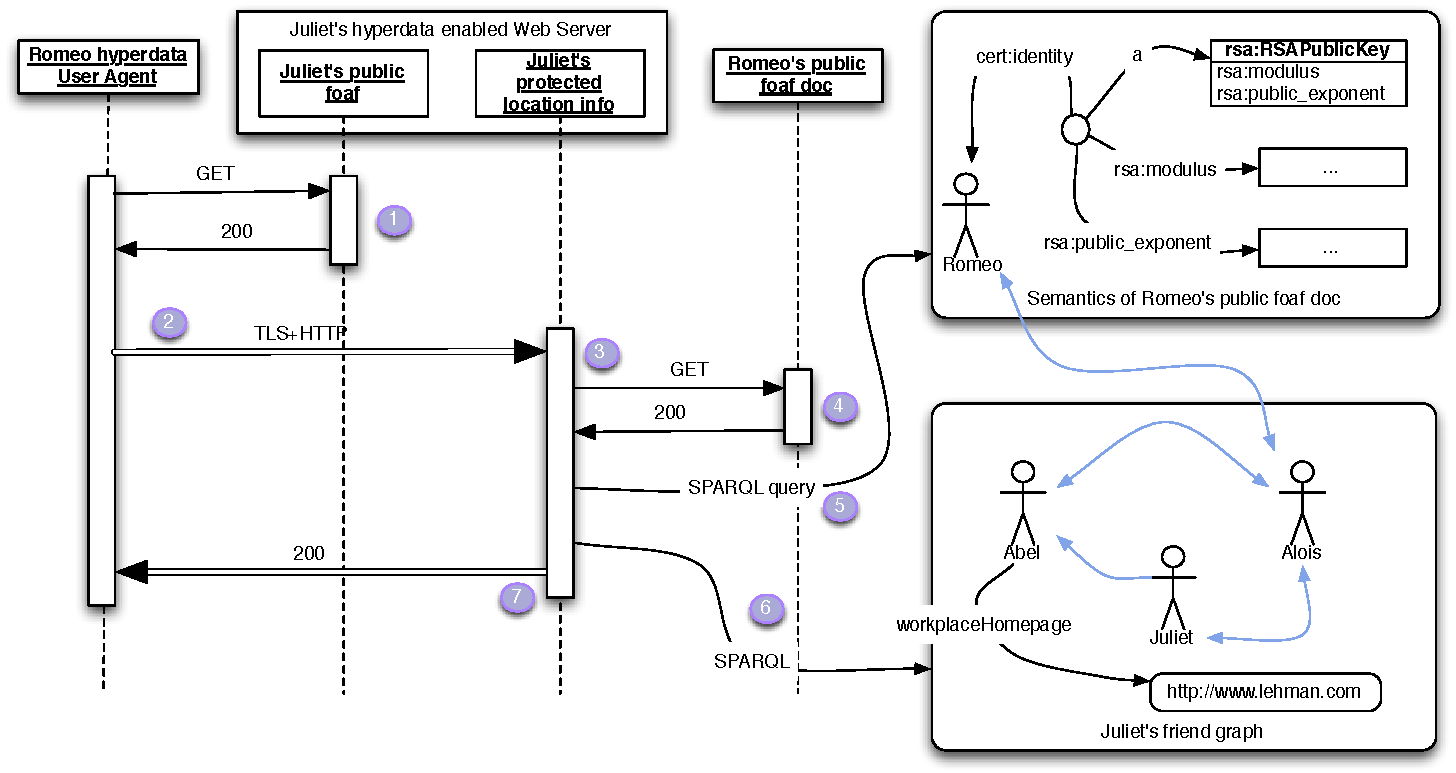
\includegraphics[width=\columnwidth]{figures/foaf_ssl_sequence}
\caption{The FOAF+SSL sequence diagram.}
\label{fig:foafsslseqdiag}
\end{figure}

The FOAF+SSL authentication protocol consists of the following steps,
as illustrated in Figure~\ref{fig:foafsslseqdiag}:

\begin{enumerate}
\item A client fetches a public HTTP resource which points to a
  protected resource, for example {\tt <https://juliet.example/location>}.
\item The client, {\tt romeo:i}, dereferences this URL.
\item During the SSL handshake, the
  server requests a client certificate. Because FOAF+SSL does not rely
  on CAs, it can ask for {\em any} certificate.  The client sends
  Romeo's certificate (which may be self-signed) containing its public
  key (see ``{\tt Subject Public Key Info}'' in
  Listing~\ref{listing:x509cert}) and a {\em Subject Alternative Name}
  URI (see ``{\tt X509v3 extensions}'' in
  Listing~\ref{listing:x509cert}).  Because the SSL handshake has been
  successful, Juliet's server knows that Romeo's client has the
  private key corresponding to the public key of the certificate.
\begin{lstlisting}[basicstyle=\rm\scriptsize\ttfamily,label={listing:x509cert},caption={Excerpt of a text representation of a FOAF+SSL certificate.}]
     Subject Public Key Info:
            Public Key Algorithm: rsaEncryption
            RSA Public Key: (1024 bit)
                Modulus (1024 bit):
                    00:b6:bd:6c:e1:a5:ef:51:aa:a6:97:52:c6:af:2e:
                    71:94:8a:b6:da:9e:5a:5f:08:6d:ba:75:48:d8:b8:
                    [...]     
                Exponent: 65537 (0x10001)
     X509v3 extensions:
           X509v3 Subject Alternative Name: 
                           URI:https://romeo.example/#i
\end{lstlisting}
\item Juliet's server dereferences the Subject Alternative Name URI
  found in the certificate and ends up with a superset of D\ref{prop:romeoSem}.
\item The document's {\em log:semantics} is queried for information
  regarding the public key contained in the X.509 certificate.  
  This can be done in part with a SPARQL query
  as shown in Listing~\ref{listing:sparqlpub}.  If the public key of
  the certificate matches the one published in the
  FOAF file, {\tt romeo:i} is authenticated.
  \begin{lstlisting}[basicstyle=\rm\scriptsize\ttfamily,label={listing:sparqlpub},caption={SPARQL query to obtain the public key information.}]
SELECT ?modulus ?exp WHERE { 
   ?key cert:identity <https://romeo.example/#i>;
        a rsa:RSAPublicKey;
        rsa:modulus [ cert:hex ?modulus; ];
        rsa:public_exponent [ cert:decimal ?exp ] .   }            
\end{lstlisting}
\item Once this authentication step is complete, the position of {\tt romoe:i} in 
  Juliet's social graph can be determined. Juliet's server can get this information
  by crawling the web starting from her FOAF file, or by other means.
\item Authentication has been done; authorization can now take place.
\end{enumerate}

\subsection{Authentication Logic}
\label{sec:authlogic}

This section draws a parallel with Section~\ref{sec:tlsauth}, again,
following the reasoning of the web server {\tt S} trying to authenticate a {\tt
  :client}.

At the end of stage 3 in the FOAF+SSL sequence diagram, 
{\tt S} has received the client certificate securely. Being
self-signed (or signed by an unknown party), its semantics are
somewhat different. {\tt S} is really only interested in the URI 
identifiers referring to the subject --- abandoning thus the limitations of DNs. 
In addition, since it is asserted by the client, {\tt S} knows that:\footnote{The signer
  being the author, following the reasoning from
  P\ref{prop:foafCertClientClaim}, P\ref{prop:sigverif},
  D\ref{def:signedCertClaim} would also end up with this result ---
  for self signed certificates only.}

\begin{customprop}{prop:foafCertClientClaim}
\begin{verbatim}
 :client :claims { <>  dc:created romeo:i; 
                       foaf:primaryTopic romeo:i.
                   romeo:i :hasPrivateKeyFor pubKey .  } 
\end{verbatim}
\end{customprop}


{\tt S} may know of {\tt romeo:i} only what it gathered from the
SSL handshake:

\begin{customprop}{prop:foafPubKey}
\begin{verbatim}
 :client :hasPrivateKeyFor pubKey . 
\end{verbatim}
\end{customprop}

When someone makes a claim, they have to agree with the logical consequences
of their claim, including those arising from new facts. Thus, someone who makes a claim {\tt :mustAgree} 
with the conclusions of the union of what we know securely, what they believe, and established reasoning rules: 

\begin{customdef}{def:mustAgree}
\begin{verbatim}
 {  ?client :claims ?clientGraph . 
  ( ?clientGrph   secureFactGraph   owlReasoningRules ) 
     log:conjunction [ log:conclusion ?C ] }
              => { ?client :mustAgree ?C  } 
\end{verbatim}
\end{customdef}

Hence, from P\ref{prop:foafCertClientClaim},
P\ref{prop:foafPubKey}, and D\ref{def:hasPrivateKeyFor}, {\tt S} may conclude that {\tt
  :client} would have to agree that it is {\tt
  romeo:i}. This should not be a surprise, as that is indeed what
one assumes someone who sends such a certificate intends.

\begin{customprop}{prop:client_IamClient}
\begin{verbatim}
 :client :mustAgree [ log:includes { romeo:i = :client  }  ] .
\end{verbatim}
\end{customprop}

Since {\tt :client} asserts it is {\tt romeo:i}, it accepts to be
inspected via {\tt romeo:i}.
Since {\tt romeo:i} is a URL, {\tt S} can dereference it and thus discover P\ref{prop:romeoSem}. 
Then, by P\ref{prop:romeoSem}, P\ref{prop:foafPubKey},
D\ref{def:hasPrivateKeyFor}, and D\ref{def:mustAgree}:

\begin{customprop}{prop:romeo_IamClient}
\begin{verbatim}
 romeo:i :mustAgree [ log:includes { romeo:i = :client  }  ] .
\end{verbatim}
\end{customprop}

In other words, both {\tt romeo:i} and {\tt :client} must agree,
given what {\tt S} knows, that {\tt romeo:i owl:sameAs :client}.  In particular {\tt romeo:i} cannot repudiate
this assertion since {\tt romeo:i} itself provided
P\ref{prop:romeoSem} authoritatively. It follows that if {\tt S} is
authorized to serve {\tt R} to {\tt romeo:i}, {\tt S} can serve {\tt
  R} to {\tt :client}.

%In other words, both {\tt romeo:i} and {\tt :client} would agree,
%given what {\tt S} knows, that they are the same. The advantage of
%this reasoning via an indirection of what others would have to agree
%to given what S knows, is that it allows {\tt S} to assert the
%minimum it needs to, and so be minimally liable.

%It follows then that if {\tt S} has to serve R to {\tt romeo:i} then
%{\tt romeo:i} cannot disagree if {\tt S} serves {\tt R} to {\tt
%:client}; this is all {\tt S} needs to know to accomplish its task.

%It is an interesting further question to find out if S also knows
%that {\tt romeo:i = :client}, but we have not at present had enough
%time to look into this.
\subsection{Following links}
\label{sec:LinkCrawling}

In the previous section, we showed how a server can authenticate
a client who claims a Web ID.  Authorization policies --- how to decide
which group of agents may access which resource --- will be particular to
each application. It could be done by giving a list of authorized Web IDs.  It could
be done by trusting statements returned by a selected group of Web IDs,
for example, when allowing all friends of a given friend access to a
resource, as specified by the representation returned by their
Web ID. This would make the initial list of trusted Web IDs similar to the trust anchors in PKI and WoT.
A lot still remains to be explored.

A topic for further research is to define the various ways in which
trust can be transmitted. Let us look at one simple example
here. Imagine a user connects to a service and is authenticated as
{\tt joe:i}, using the FOAF+SSL method described above. Imagine {\tt
  joe:i} returns a representation claiming {\tt joe:i owl:sameAs
  romeo:i}. Since anyone could make that statement, that, in itself,
should not be the basis for belief for services that care about
security. If, on the other hand, {\tt romeo:i :semantics [
    log:includes \{ romeo:i owl:sameAs joe:i . \} ]}, then this could be
used as confirmation of the claim, and from there on both IDs could be used 
interchangeably by {\tt S}.

\section{Related work}
\label{sec:other}

%FOAF+TLS builds on
%a number of existing proposals and implementations of various authentication
%systems. More specifically, FOAF+TLS relies on the TLS layer to authenticate the client (that is, to verify that 
%the remote client is indeed in possession of the private key corresponding to this certificate)
%and on the Web to authenticate the identity claim made by the client in its certificate.

Unlike the OpenPGP extension to TLS~\cite{rfc5081}, which also aims to
rely on a Web-of-Trust by using PGP certificates instead of the usual
X.509 certificates, FOAF+SSL makes only slight changes in the way
X.509 certificates are used; it does not require changes in the actual
SSL stack. With the OpenPGP TLS extension, the problem of key distribution 
still remains. Public PGP keys can be stored on public key servers, but there is no
global dereferencing mechanism for finding a key, as there is in the FOAF+SSL protocol.

OpenID also shares considerable similarities with FOAF+SSL, due in
part to OpenID's reliance on URLs as identifiers, just as FOAF+SSL
relies on dereferenceable URIs bearing FOAF data. However, OpenID fails to
make much use of the information at the OpenID resource, using it only
to find the authorization service. As a result, OpenID requires a much
higher number of connections to establish identity ---~6 as opposed to
2~--- and parts ways with RESTful design in the attribute exchange
protocol, loosing thereby the advantages of a networked architecture.

\section{Conclusions}

FOAF+SSL provides a secure and flexible global
authentication system.  With public key cryptography at its core, it gains all the
security advantages of this technology.
Because FOAF+SSL is RESTful and integrates well with the Semantic Web, 
it can discover more information about an entity by walking the Linked Data cloud.  Compared with PKI,
FOAF+SSL removes the need for hierarchical authorities to assert
identity, making it much more flexible.  Thus, this
mechanism adapts itself well to the formation and expansion of virtual
organisations and distributed social networks.

%% Not sure where to stuff these acknowledgements, but I've listed them.

\section*{Acknowledgements}
{
\footnotesize
Ian Jacobi acknowledges funding for this project from NSF Cybertrust award \#0524481 and IARPA award \#FA8750-07-2-0031.
Bruno Harbulot acknowledges EPSRC funding under grant EP/E001947/1 (\url{http://www.nanocmos.ac.uk/}).
}

\bibliographystyle{splncs}
\bibliography{spot2009,rfc}


\end{document} 
